\documentclass[11pt]{article}

\usepackage{fullpage}
\usepackage{amsfonts}
\usepackage{graphicx}

\def\eq1{y=\frac{x}{3x^2+x+1}}

\begin{document}
The set of natural numbers is denoted by $\mathbb{N}$. 

The set of integers is denoted by $\mathbb{Z}$.

The amsfonts allows advanced math notations. 

Macros is custom commands. $\subset$

$\eq1$

Identify the asymptotes for the graph of $\eq1$.

Graphics need the graphics package- graphicx.
Use includegraphics fucntion. scale, width or angle can be specified.
Only png,jpg,gif,pdf supported.
\begin{center}
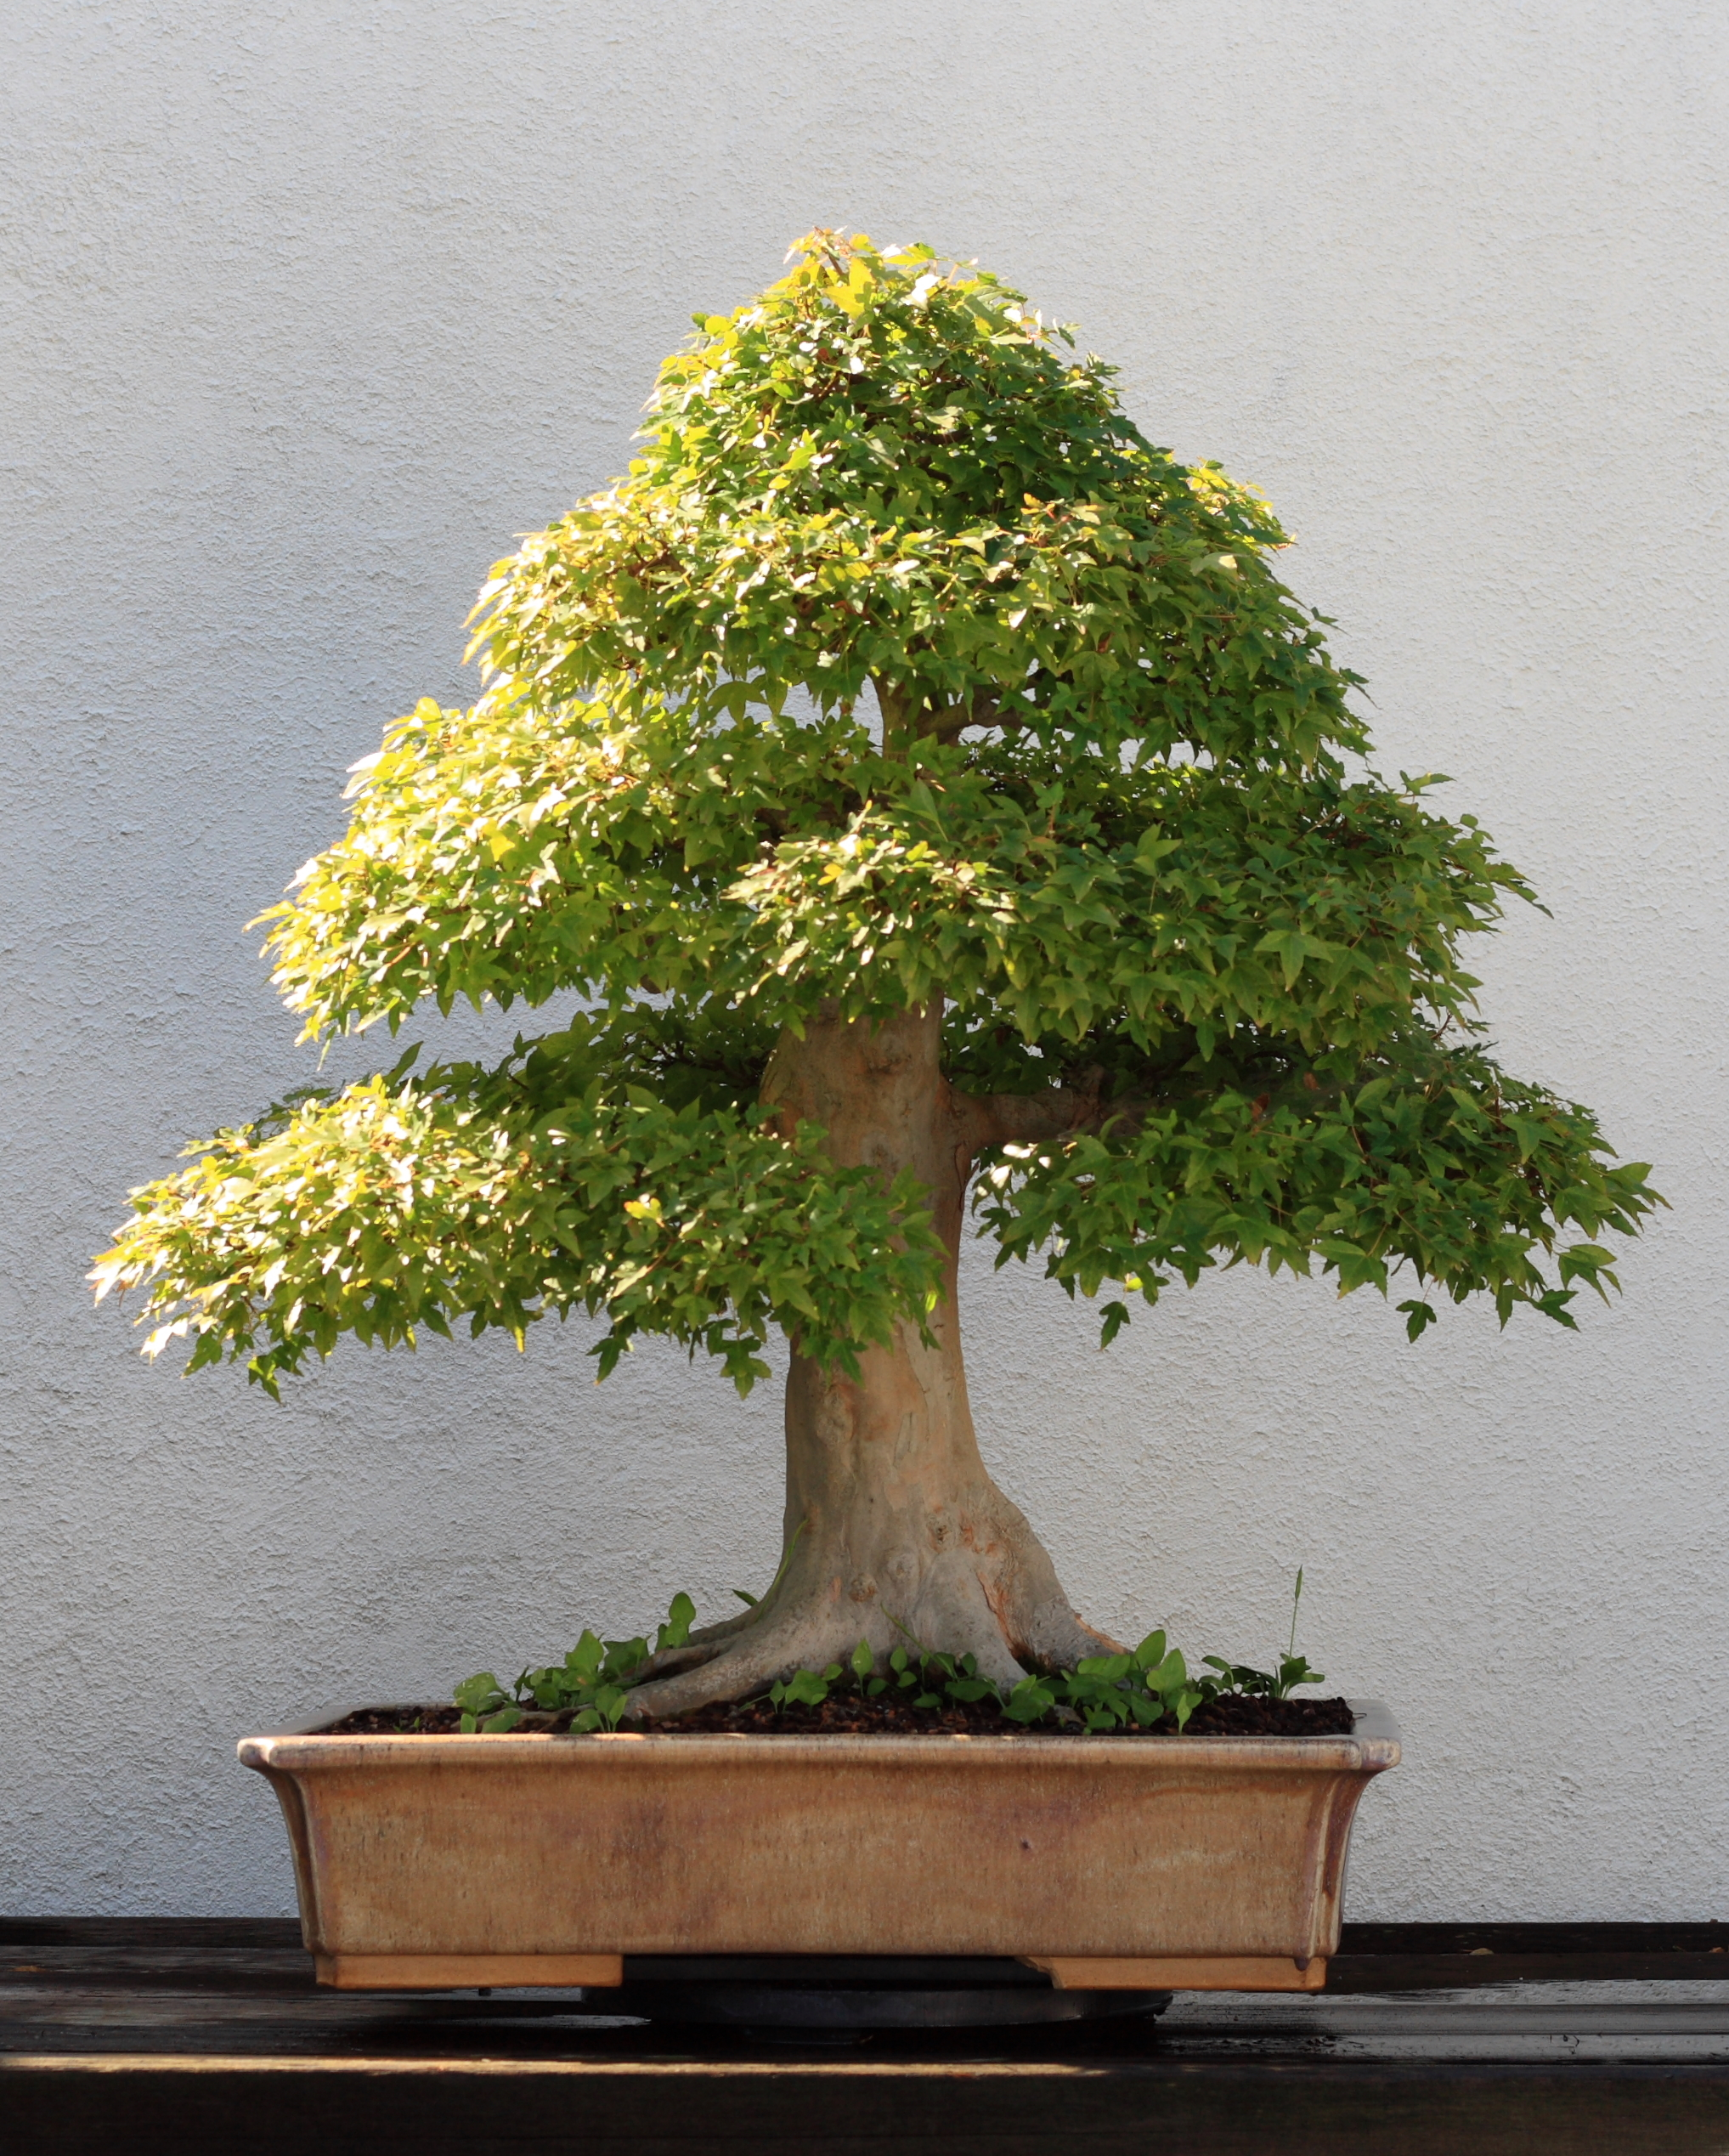
\includegraphics[scale=.15, angle=180]{e7a7b29f11bd0643661ba1611b5c62a4.jpg}
\end{center}

\end{document}